\chapter{Discretización de sistemas}

\section{Enmascaramiento de frecuencias}


\section{Método de Euler - diferencia en adelanto}

Se remplaza $S$ por:  

\begin{equation}
    S = \frac{z-1}{h}
\end{equation}

En la Figura \ref{fig:euler} se observa la transformación del semiplano negativo de $S$,
por método de Euler. En general, este método se utiliza para discretizar los integradores.

\begin{figure}
    \centering
    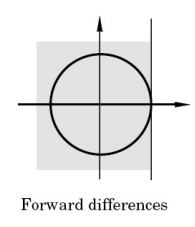
\includegraphics[width=.3\textwidth]{img/Euler.png}
    \caption{Transformación del semiplano negativo de $S$, por método de Euler.}
    \label{fig:euler}
\end{figure}

\section{Diferencia en ataso}

Se remplaza $S$ por: 

\begin{equation}
    S = \frac{z-1}{zh}
\end{equation}

En la Figura \ref{fig:atras} se observa la transformación del semiplano negativo de $S$.
En general se utiliza para transformar los derivadores.

\begin{figure}
    \centering
    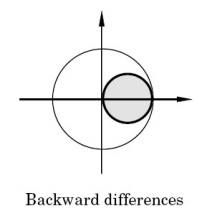
\includegraphics[width=.3\textwidth]{img/atras.png}
    \caption{Transformación del semaplano negativo de $S$, por diferencias en atraso.}
    \label{fig:atras}
\end{figure}

\section{Método de Tustin, bilineal}

Se remplaza $S$ por: 

\begin{equation}
    S = \frac{2(z-1)}{h(z+1)}
\end{equation}

Esta transformación tiene la caracteristica de conservar la estabilidad del sistema. 
En la Figura \ref{fig:tustin} se observa la transformaciónd el semiplano $S$. 

\begin{figure}
    \centering
    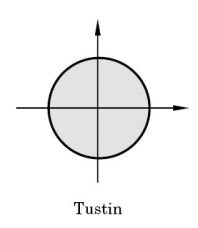
\includegraphics[width=.3\textwidth]{img/tustin.png}
    \caption{Transformación del semiplano negativo de $S$ por el método de Tustin.}
    \label{fig:tustin}
\end{figure}

\section{Discretización por mantenedor de orden cero (ZOH)}

La discretización por el mantenedor de orden cero (ZOH) es ampliamente usada, ya que es 
forma que se discretiza al sensar un sistema continuo. Su análisis es más complejo que en los casos anteriores, 
esto puede observar en la Figura \ref{fig:zoh}. La ecuación para obtener $G(z)$ esta dada por Ecuación \ref{eq:zoh}.

\begin{figure}
    \begin{tikzpicture}[auto, node distance=3.5cm, auto, >=latex']
     % We start by placing the blocks
     \node [input, name=input] {};
     \node [block, right of=input] (dac) {DAC};
     \node [block, right of=dac] (system) {$G(s)$};
     \node [block, right of=system] (adc) {ADC};
     \node [output, name=output, right of=adc] {};

     % Once the nodes are placed, connecting them is easy. 
     \draw [draw,->] (input) -- node {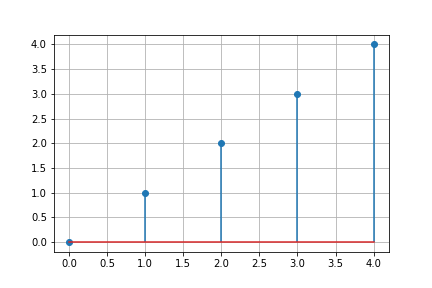
\includegraphics[width=100px]{img/xk.png}} (dac);
     \draw [->] (dac) -- node {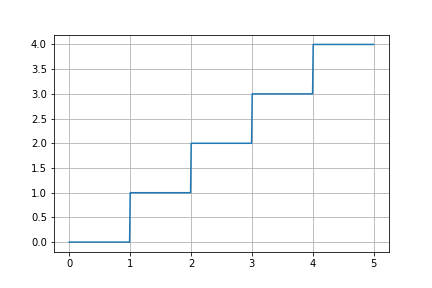
\includegraphics[width=100px]{img/dac.png}} (system);
     \draw [->] (system) -- node {$Y(s)$} (adc);
     \draw [->] (adc) -- node {$Y(z)$} (output);
\end{tikzpicture}
    \caption{Sistema con ZOH}
    \label{fig:zoh}
\end{figure}

\begin{equation}
    \label{eq:zoh}
    G(z) = (1 - z^{-1}) Z \left\{ 
        \mathcal{L}^{-1} \left\{ 
            \frac{G(s)}{s}
        \right\}_{t=hk}
    \right\}
\end{equation}

\section{Determinación de $h$}

La correcta determinación de $h$ es fundamental para un buen funcionamiento del sistema. Si bien no existe una teorema para determinar $h$, como si sucede con el teorema de muestreo, 
una regla practica es tomar el producto $\omega_c h$ entre $0.15$ y $0.5$, donde $omega_c$ es el ancho de banda de la respuesta al impulso a lazo cerrado (preguntar que es $\omega_c$).